\documentclass[10pt,twocolumn]{IEEEtran11}

\usepackage{comment}
\usepackage{times}
\usepackage{epsfig}
\usepackage[T1]{fontenc}
\usepackage[utf8]{inputenc}
\usepackage{graphicx}
\usepackage{subfigure}
\usepackage{url}
\def\BibTeX{{\rm B\kern-.05em{\sc i\kern-.025em b}\kern-.08em
    T\kern-.1667em\lower.7ex\hbox{E}\kern-.125emX}}

\oddsidemargin -15pt
\evensidemargin -15pt
\leftmargin 0 pt
\topmargin -35pt
\textwidth = 6.9 in
\textheight = 9.1 in

\newcommand{\itembase}{\setlength{\itemsep}{0pt}}
\newcommand{\eg}{{\it e.g., }}
\newcommand{\ie}{{\it i.e., }}
\graphicspath{{FIG/}}

\begin{document}
\bibliographystyle{IEEE}

\title{\Large \bf Assessing Connectivity Bias in the Twitter Network
%\thanks{
}

\author{Adam Bates and Lara Letaw\\
Department of Computer \& Information Science\\
University of Oregon\\
\textit{\{amb,zephron\}@cs.uoregon.edu}}

\maketitle
% You have to do this to suppress page numbers.  Don't ask.
\pagestyle{empty}
\begin{abstract}
Over the past few years Twitter has been at the forefront of the online social networking phenomenon.  Twitter experienced a growth rate of almost 1400\% between February 2008 and February 2009~\cite{lrossi:mcgiboney_twitters_2009}.  This surge in popularity has legitimized Twitter as a channel for communities to interact within the United States and across the globe.  Still in its nascent stages, there is much at that is unknown about the nature of interaction and influence within the Twitter network.\\
This paper presents a detailed analysis of the nature of the relationships that exist between users within an online social network.  We have collected a complete subgraph of the Twitter network that contains tens of millions of users and hundred of millions of those users' relationships.  We profile this subgraph and explore its strengths and limitations by comparing it to a random sample of Twitter users.  We then characterize the connectivity of our dataset based on the user attributes associated with each Twitter account.  We use these results to identify a number of bias patterns that can be observed between different user groups.  It is our belief that these observations shed new light on the nature of the global community's Twitter usage.\\
\end{abstract}

\begin{keywords} 
Online social network, Twitter, Measurement, Overlay topology
\end{keywords}

\section{Introduction}
\label{sec:introduction}
Twitter is a microblogging and social networking servive that allows its users to send short, one-to-many messages called \textit{tweets}.  Like many online social networks, users can opt-in to viewing other users' messages \textit{following} them, creating a customized content stream.  The act of following is an implicit endorsement of another user on the network.  It can be inferred that the user being followed is of interest to another user on the network.  These interactions constitute a networked system through which users connect and message propagate.

In order to gain a better understanding of Twitter, it is necessary to investigate the nature of this network.  This information can be used when considering design decisions or allocating resources within Twitter or other future social networks.  While Twitter is innovative in the manner in which it distributes messages, a great deal of this profiling must take place at the user-level network.

Twitter, like many other online social networks, present a novel opportunity to study interactions between people.  Through them, it becomes possible to easily quantify the activities of millions.  The simple and open structure of the Twitter network is particularly well-suited for this purpose.  As each user account is associated with a variety of attributes, there a variety of methods to approach this task.  The work we present here establishes a framework for further analysis.

There are many commonly held intuitions regarding influence that can be proved, disproved or measured through analysis of Twitter.  For example, it is a commonly held belief that activity in states such as California and New York is of a higher culturally relevance than the activity in other states.  As each user account is associated with a location field, it is possible to use the Twitter network to measure the influence of these allegedly trend-setting states.  Other, subtler biases can also be identified and evalued in the same manner.

A defining aspect of Twitter that lends itself to research is that all activity defaults to public.  Each user's messages are visible unless they explicitly change their privacy setting.  Although tweets can be protected, all other information associated with an account visible to all.  Using this publicly available connectivity information, it is possible to make broad assessments of connectivity within the Twitter community.

Given the massive size and continued growth of Twitter, capturing a complete snapshot of the network is an increasingly unrealistic endeavor.  To make matters worse, Twitter imposes prohibitive rate limitations on access to many of its network measurement resources.  It is therefore necessary to obtain a representative and meaningful sampling of the network before analysis begins.

One possible option is to take a random sample of a small percentage of Twitter accounts and activity.  Inspection of this random sample's attributes would lead to a representative view, but not necessarily a meaningful one.  The users of greatest interest are small in number and some of their attributes will have extreme values.  A random sample is not likely to capture these users' impact on the network.

It is also possible to conduct a biased sampling.  Here, interesting users with extreme user attribute values are specifically targetted for measurement.  If good metrics are used to assess influence, this will ensure that important user accounts are not crowded out by unimportant ones.  Of course, this leads to data that is less representative than a random sampling.  It can be observed that there is a natural trade-off between these two goals.

Our approach finds a healthy compromise between these competing priorities by starting with a biased sample and then performing a mult-hop crawl across a small piece of the network to conduct further sampling.  This crawl creates a snapshot of a part of Twitter that is acceptably representative while simultaneously ensuring that rare users are acceptably prominent.  We establish that our snapshot is representative by comparing its profile to the profile of a true random sample.

STILL NEED TO PUT A SUMMARY OF OUR WORK APPROACH AND MAIN FINDINGS HERE (AS PER REZA'S REPORT DESCRIPTION)

The rest of this paper is organized as follows.  We outline our data collection process in section \ref{sec:datacollection}.  In section \ref{sec:methodology}, we present our method for evaluating connectivity bias within the Twitter network.  Analysis of our results is contained in section \ref{sec:analysis}.  We review some of the related work in section \ref{sec:relatedwork}.  Section \ref{sec:conclusion} concludes the paper.

\section{Data Collection}
\label{sec:datacollection}
At the start of our work we inherited a large dataset from Rejaie \textit{et all} that was created through a biased sampling of the Twitter network.  The dataset contained partial connectivity information for 242,275 potentially influential users.  Due to limitations of the Twitter REST API at the time of collection, the connectivity data was incomplete.  Additionally, the dataset did not include the associated attribute information for each user because it was not germaine to Rejaie's previous work.  This dataset needed to be completed before beginning our analysis.

Our goal was to characterize the relationships in a completed section of the Twitter network.  It was first necessary to determine if a large, complete subgraph existed within this dataset.  A collection of smaller subgraphs would not be sufficient as they would be less likely to capture the impact of rare influential users.  By performing a series of reconstructions of the graphs in the dataset we were able to discover a subgraph of 215,606 sampled users.  Including the next hop information for these sampled users, the subgraph included 15,548,091 unique user accounts.

The inherited dataset was not originaly intended to measure the extreme connectivity degrees of rare users.  As a result, the friend and follower counts for each user in the subgraph were truncated at 1,000.  This truncation was due to the prohibitive rate limiting of of the Twitter API, which made it infeasible to collect the complete connectivity information for these users in real time.  Over the course of several weeks, we were able to restore this missing information.  Several months passed between these two collection phases.  The potential error that this introduced is explored below.

Simultaneously, we needed to collect the user attribute information for the tens of millions of users in our subgraph.  Completing this task via the Twitter API was difficult due to the connectivity restoration process, and it was not our wish to violate Twitter's terms of service by launching API calls from dozens of hosts.  Fortunately, we were able to find an alternate method of collecting user attribute information.  Twitter provides XML dumps of user information through their primary website.  These calls are not subject to API rate limites, presumably for the benefit of mobile applications that may issue frequent user lookups.  Using this service, we were able to collect the necessary information without violating the Twitter API ToS.

\subsection{Measuring Error}

Because our user attribute information was collected in less than a month, we have assumed that no significant error is present.  It is not possible to capture a realtime snapshot of user attributes in the Twitter network, so we have no method of comparing collected attributes to actual attributes.  Our intuition here is that most user attributes are not subject to frequent change.  The exception to this is friend and follower count, which is explored below.  For our purposes, the collected user attribute information can be accepted as accurate.

In contrast, connectivity information for our subgraph was collected in two different phases between September 2010 and February 2011.  It would be foolish to assume that significant change did not occur in the network over this time.  It was therefore necessary to confirm that the temporally disparate collection phases did not introduce error to our network measurements.  To do this, we compared our snapshot of connectivity for each user to the stated friend and follower counts in each user's attributes.

GRAPHIC for FOLLOWERS: The CDF I am working on that shows the error percentage for our core users between actual degree and measured degree.

GRAPHIC for FRIENDS: The CDF I am working on that shows the error percentage for our core users between actual degree and measured degree.

Figures \ref{fo-cdr} and \ref{fr-cdr} confirm that we have captured an accurate view of connectivity in our piece of the Twitter network.  90\% of users blah blah blah.  This speaks to the general stability of the social network that Twitter facilitates.

(Q: Plotting the growth of this subgraph -- would this be a neat consideration for future work?  Not that we need to do it, but we can always suggest it in the paper for the benefit of Team Reza)

\subsection{Profiling}

Our set of Twitter users was selected by first selecting 250,000 id's of users that met a certain time-in-system threshold, and then querying the Twitter API for all users connected to that initial core.  Since user connectivity is central to our study, this allowed us to quickly acquire a subgraph in which every node was usable.  However, since this collection method was not random, the distribution of attributes across our dataset could be different than that which we would observe by choosing random users.  These differences are important to examine because they may indicate ways that our dataset is not generalizable to the entire Twitter universe.

To quantify these potential discrepancies, we perform attribute profiling both on our connected subgraph and on a set of 1.5 million randomly-selected users.  We simply calculate the percentages of users falling into each attribute basket for each set, and compare.  In order to express to what extent our selection of the inital core users may have influenced the profile of the entire subgraph, for some attributes we also include distributions for the original 250K.

\subsubsection{Boolean Attributes}

Two of the attributes we examined were true/false values: protected and geo-enabled.  Below is a table of percentages of users who enabled each attribute, for the core, connected, and random data sets.

[table of percentages for boolean attribs]

We find that our core users were less than half has likely to be protected, and more than three times more likely to allow the inclusion of GPS information in their tweets than the random users.  The percentage of geo-enabled users in the connected subgraph is in between that of core and random, which indicates that the original user selection could have carried over to the first-hop connections to some extent.  Interestingly, the subgraph users are more likely than either of the other sets to be protected.  This may be because users who are connected to the initial group, which we would characterize as more ``established", are more experienced than the average random user, as random users likely include many people who have signed up but have not made much use of their accounts.  The random set could, for example, include users who are not connected to anyone else.

\begin{figure}[h]
 \centering
 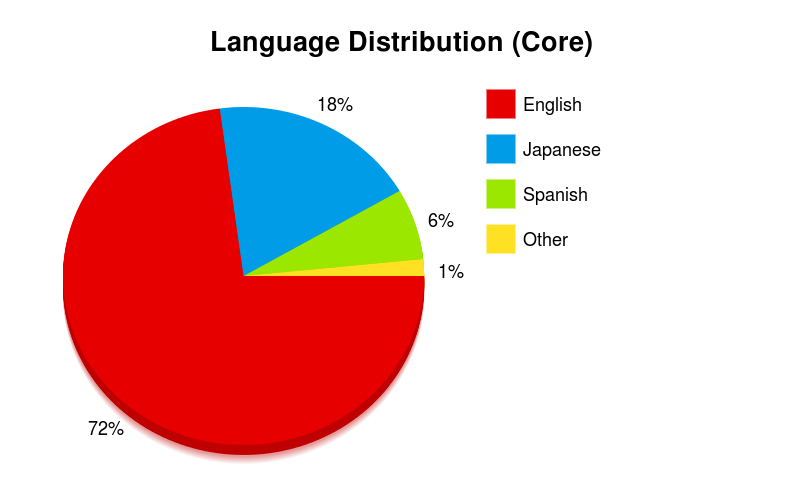
\includegraphics[bb=0 0 800 500,scale=.2]{./images/lang-core.png}
 % lang-core.png: 800x500 pixel, 72dpi, 28.22x17.64 cm, bb=0 0 800 500
 \caption{For the core set, the percentage users who have marked Japanese as their Twitter language is more than four times that of the random set.}
\end{figure}

\begin{figure}[h]
 \centering
 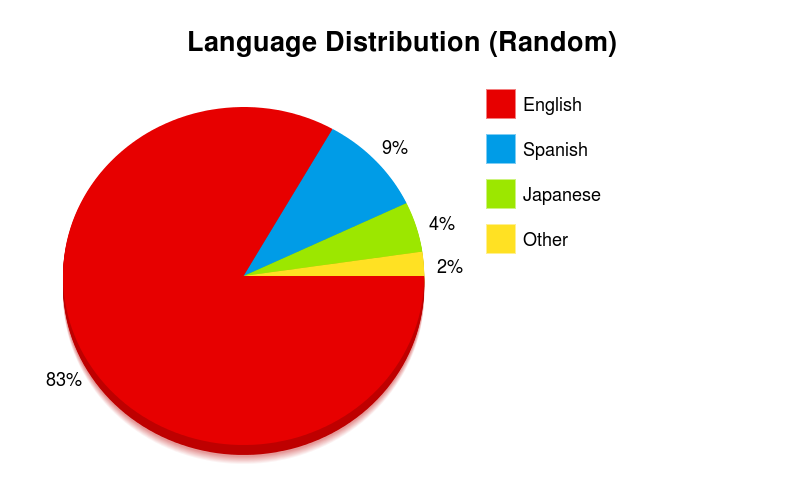
\includegraphics[bb=0 0 800 500,scale=.2]{./images/lang-rand.png}
  % lang-rand.png: 800x500 pixel, 72dpi, 28.22x17.64 cm, bb=0 0 800 500
 \caption{English, Spanish, and Japanese are the top languages for both the connected and the random user sets.}
\end{figure}

\subsubsection{Language}

Users have seven choices for the language attribute.  Choice of language affects the text of the Twitter interface, but does not translate tweets.  It is unclear whether the language changes based on the location (IP address) of the user, or if English is default for everyone.  We find that, in comparison to the random set, the connected and core users are substantially more likely to be configured for using Japanese.  This could indicate that the filtering techniques used to gather our original set of users was more likely to pick up Japanese users.

[language table]

\subsubsection{Location}

Say how it lines up well with the census, too.

\begin{figure}[t]
 \centering
 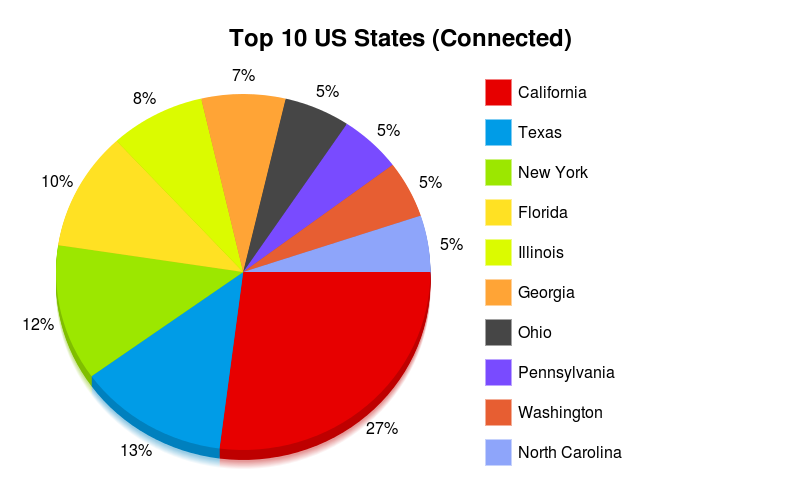
\includegraphics[bb=0 0 800 500,scale=.2]{./images/loca-conn.png}
 % loca-conn.png: 800x500 pixel, 72dpi, 28.22x17.64 cm, bb=0 0 800 500
\caption{}
%\end{figure}

%\begin{figure}
% \centering
 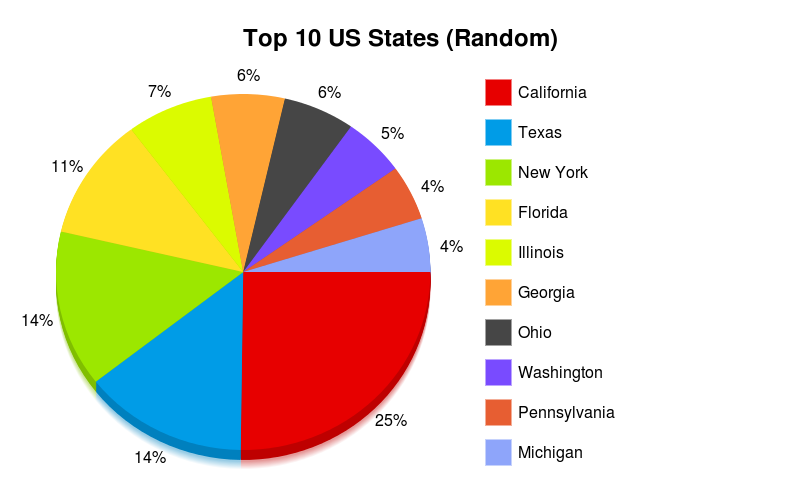
\includegraphics[bb=0 0 800 500,scale=.2]{./images/loca-rand.png}
 % loca-rand.png: 800x500 pixel, 72dpi, 28.22x17.64 cm, bb=0 0 800 500
\caption{}
%\end{figure}

%\begin{figure}
% \centering
 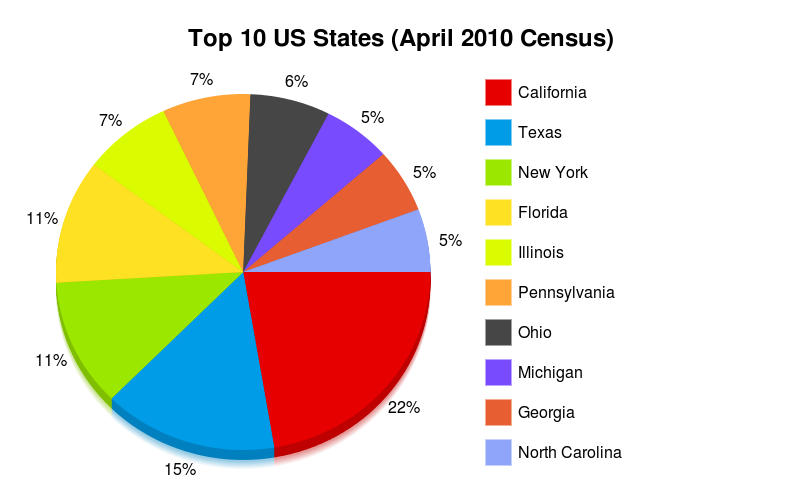
\includegraphics[bb=0 0 800 500,scale=.2]{./images/loca-actu.png}
 % loca-actu.png: 800x500 pixel, 72dpi, 28.22x17.64 cm, bb=0 0 800 500
\caption{The distribution of U.S. states for both the random and the connected datasets aligns well with the population census data.}
\end{figure}

\subsection{Approaching Attribute Analysis}

\subsubsection{Location}

The location attribute field has no enforced format, apart from length.  That is, users can type in essentially any text for their location.  From a small random sample and manual examination of this attribute field, we estimate that approximately 50\% of users provide location text that can be matched to at least one city, state/region, or country.  We also find that almost 90\% of users who match one city will match more than one city.  Since we want our analyses to be by specific location, we need to address these ambiguities.

\begin{figure*}[t]
 \centering
 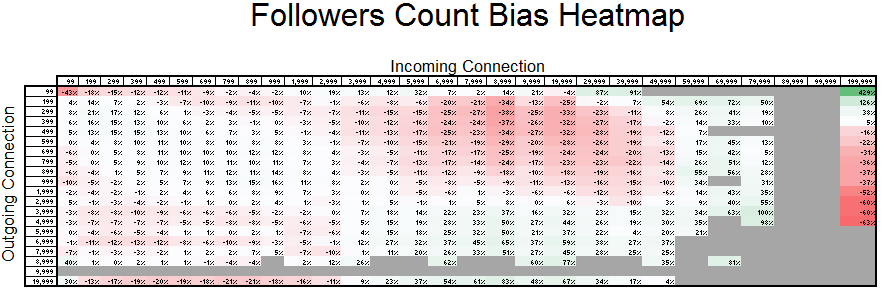
\includegraphics[bb=0 0 664 222,scale=.62]{./images/followers_count.png}
 % followers_count.png: 885x296 pixel, 96dpi, 23.42x7.83 cm, bb=0 0 664 222
 \label{fig:follower_count}
 \caption{A connectivity bias chart for number of followers in logarithmically increasing groupings.}
\end{figure*}

\begin{figure*}[t]
 \centering
 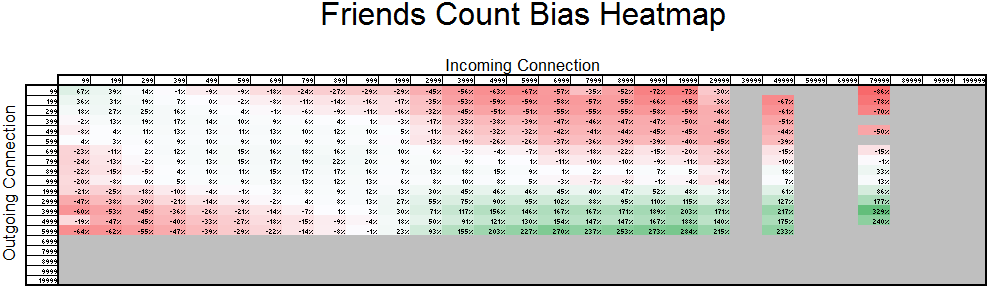
\includegraphics[bb=0 0 746 221,scale=.55]{./images/friends_count.png}
 % friends_count.png: 995x294 pixel, 96dpi, 26.33x7.78 cm, bb=0 0 746 221
 \label{fig:friend_count}
 \caption{A connectivity bias chart for number of friends in logarithmically increasing groupings.}
\end{figure*}


Given that there are hundreds of thousands of cities in the world, we decided to start our location analyses with U.S. states because of their familiarity to the authors.  Our approach is to filter users based on exact matches with a pre-compiled list of U.S. cities in the standard \textit{San Francisco, CA} or \textit{San Francisco, California} format.  If a user matches one of these locations exactly, the user cannot exactly match a different location.  For the top 100 most populous cities, we try to match the city name itself, without the state, with the intuition that, for example, users from \textit{San Francisco} would not find it necessary to specific their state.



\section{Methodology}
\label{sec:methodology}
\subsection{Approaching Attribute Analysis}

Paragraph: Describe the manner in which we approach each attribute.  Explain that for some attributes with a small number of options it is easy to investigate all simultaneously.  Explain for the range options that we created logarithmic bins to accurately capture our extreme uses.\\

Paragraph: Explain how Location was an entirely different animal because it is a freely entered text field.  A large number of users do not put valid locations in this field.  For the users that do, those options are often difficult to parse.\\

Paragraph:  Mention that some attributes were not considered at all.  Explain the attributes that were not considered because they were completely irrelevant (bg color)  Explain the attributes that were not considered because their values were not sufficiently heterogenous (verified).\\

Paragraph: Mention the simple random survey of records that was performed, the percentage of users with no entry, the percentage of users with an indecipherable entry, etc.\\

Paragraph: Explain that it was decided to evaluate location based on state.\\

\subsection{Evaluation}

Paragraph: Explain the basic challenge of deriving bias from the measured following patterns.

Paragraph: Explain the method for calculating the expected connectivity in a randomized, bias-free version of our subgraph.  Include formula.

Paragraph: Explain the method for calculating bias from this value and the measured values.  Include formula.



\section{Analysis}
\label{sec:analysis}
Paragraph -- introduce results. \\

\subsection{System Age}
\subsection{State}
\subsection{UTC Offset}
\subsection{Language}
\subsection{Geo-Enabled}
\subsection{Protected}
\subsection{Follower Count}
\subsection{Friend Count}
\subsection{Statuses Count}
\subsection{Listed Count}

Include commentary on what the graphs tell us throughout.\\

Conclude that across these attributes there are several identifiable patterns -- similar users follow eachother, dissimilar users follow eachother, low degree users follow high degree users, extreme low degree users deviate from general usage, extreme high degree users deviate from general usage.  Identify which attributes belong to which patterns.\\

\section{Related Work}  
\label{sec:relatedwork}
One of Twitter's core functions is the analysis of individual messages to determine trending topics.  As such, Twitter is capable of acting a cultural barometer.  A variety of studies have attempted to answer the question of how information spreads within the Twitter network.  Investigations have included spam, the meme life cycle, and news discovery and explanation.\\\\
A variety of Twitter-related work has been conducted over the past several years.  The majority of this work focuses on the analysis and propagation of individual messages as they spread through the network.  Cheng \textit{et al} have used tweets to attempt to geo-locate users based on the content of their messages ~\cite{CCL10}.  Lerman and Ghosh have studied Digg and Twitter to measure news items' lifespan and speed within social networks ~\cite{LG10}.  Sadikov and Martinez have conducted similar work, chosing instead to focus on URL and tag propagation ~\cite{SM09}.\\
It is only reasonable that message-level analysis has captured the attention of the research community.  After all, the novelty of modern social networks is largely that they are a new medium for the spread of information.  For the purposes of assessing influence, however, message-level analysis does not tell the whole story.  Much of this work lies in predictive message filtering or spotting trending phrases.  This is not perfectly suited for the task of broadly determining who is influencing who.  Instead, we ask a much simpler question -- what type of people are users choosing to listen to?\\
For this, we turn to user-level analysis.  When a user choses to opt-in to another user's tweet stream, this says much more about influence than the propagation of individual messages.  This idea of influence through followers is a truth that rests at the very core of Twitter, one that can be plainly seen by visiting any user's page and making note of the prominently displayed ``Follower'' and ``Following'' numbers.  Our contribution will be to take this fundemental concept and cross-reference it with various user attributes in an attempt to make more general claims about the nature of influence in the Twitter network.

\section{Conclusion}
\label{sec:conclusion}
In this paper we have presented a detailed analysis of a large subgraph of the Twitter network.  We have identified a number of influence patterns across different attributes within the twitter network.  Our work is unique in that it provides a method of tracking information flow without being dependant on access to individual messages.  There are a number of pitfalls to message analysis that our work avoids.  It is our belief that a combination of both methods of Twitter network analysis are necessary in order to gain a complete perspective on the way this tool is used.\\

Future work -- ideas to consider regarding future projects that could come of our work?\\

\bibliography{./citations.bib}

\onecolumn
\appendix{User Attributes}
\label{app:user-attributes}
Below are the user attributes we plan to examine in our analyses. In reference to number of baskets, \textit{varied} means we will experiment with different numbers of baskets.\\

\noindent \begin{tabular}[t]{| p{1in} | p{1.75in} | p{1in} | p{1in} | p{1.25in} |}
\hline
\textbf{Attribute} & \textbf{Description} & \textbf{\# of Baskets (Core)} & \textbf{\# of Baskets (All)} & \textbf{Values}  \\ \hline
Location & User-reported geographic location. & 3481 & 3481 & U.S. state code \\ \hline
Protected & If true, only approved followers may see the user's tweets & 2 & 2 & true, false \\ \hline
Followers Count & Number of users who track this user's tweets & 2116 & 2116 & integer \\ \hline
Friends Count & Number of users this user follows & 2116 & 2116 & integer \\ \hline
Account age & Difference between account creation date and current date & 169 & 169 & time \\ \hline
\begin{comment}
UTC Offset & Time offset from Coordinated Universal Time & 34 & 34 & integer \\ \hline
Time Zone & Logitudinal region & 141 & 143 & time zones  \\ \hline
\end{comment}
Geo-Enabled & GPS meta data is included on tweets & 2 & 2 & true, false \\ \hline
Verified & Twitter has verified the identity of the user, currently used for Twitter partners and advertisers & 2 & 2 & true, false \\ \hline
Statuses Count & Number of tweets & 2116 & 2116 & integer  \\ \hline
Language & User's chosen language & 7 & 7 & en, de, it, es, ja, fr, ko \\ \hline
Contributors Enabled & If enabled, multiple users can tweet from this account & 2 & 2 & true, false \\ \hline
Listed Count & Number of lists that include this account & 2116 & 2116 & integer \\ \hline
Show All Inline Media & Display photos and videos of other users, not just friends & 2 & 2 & true, false \\ \hline
URL & This user posted a URL & 2 & 2 & true, false \\ \hline
Is Translator & User has signed up to translate other people's tweets  & 2 & 2 & true, false \\ \hline
%Status Source & Where the most recent status was tweeted from & 5,144 & 39,566 & (none), web, various URLs \\ \hline  
\end{tabular}

\section{Dataset Profile}

\textit{Available users} are those for which user profile data was successfully collected.  Unavailable users are those for whom an attempt to acquire user attributes resulted in a \textit{404 Not Found} error.  We assume these user accounts are closed.\\ 
\begin{tabular}[t]{| l | l |}
\hline
Users & 17,688,493  \\ \hline
Available Users & 17,475,570 (98.8\%) \\ \hline
Unavailable Users & 212,923 (1.2\%) \\ \hline
Core Users & 242,275 \\ \hline
Available Core Users & 238,323 (98.8\% of core) \\ \hline
Unavailable Core Users & 3,952 (1.2\% of core) \\ \hline
\end{tabular}

\subsection{Subgraphs}
\textit{Graph edges} refers to the connections between core users and any other user.\\\\
\begin{tabular}{| l | l | }
\hline
Users is Subgraph 1 & 15,548,091 \\ \hline
Available Users is Subgraph 1 & 15,363,277 \\ \hline
Core Users in Subgraph 1  & 194,004 \\ \hline
Remaining Core Users  & 48,267 \\ \hline
Remaining Subgraphs  & 46,403 \\ \hline
Connections to Subgraph 1  & 46,924 \\ \hline
Total Connected Users & 240,932 \\ \hline
\end{tabular}

\subsection{Boolean User Attributes}
Attributes whose values are either \textit{true} or \textit{false}.\\\\
\begin{tabular}{| l | l | l |}
\hline
\textbf{Attribute} & \textbf{\# True (Core)} & \textbf{\% True (Core)} \\ \hline
Protected & 8,517 & 3.575  \\ \hline
Geo-Enabled & 58,432 & 24.518 \\ \hline
Verified & 119 & 0.050 \\ \hline
Contributors Enabled & 7 & 0.003 \\ \hline
Show All Inline Media & 18,870 & 7.918 \\ \hline
URL & 118,364 & 49.665 \\ \hline
Is Translator & 72 & 0.030 \\ \hline
\end{tabular}

\subsection{Enumerated User Attributes}
Attributes for which there are a relatively small number of values, other than boolean values.
\subsubsection{Language}
Percentage of users per language.\\\\
\begin{tabular}{| l | l | l | l | }
\hline
\textbf{Language Code} & \textbf{Language} & \textbf{\# (Core)}  & \textbf{\% (Core)} \\ \hline
en & English & 173,782 & 72.919 \\ \hline
ja & Japanese & 44,499 & 18.672 \\ \hline
es & Spanish & 16,210 & 6.802 \\ \hline
de & German & 1,560 & 0.655 \\ \hline
fr & French & 1,222 & 0.513 \\ \hline
it & Italian & 713 & 0.299 \\ \hline
ko & Korean & 337 & 0.141 \\ \hline
\end{tabular}

\subsubsection{UTC Offset}
\begin{tabular}{| l | l | l |}
\hline
\textbf{UTC Offset} & \textbf{\# (Core)} & \textbf{\% (Core)} \\ \hline
(none)	&	38287	&	16.065	\\ \hline
32400	&	36551	&	15.337	\\ \hline
-18000	&	26196	&	10.992	\\ \hline
-10800	&	25001	&	10.490	\\ \hline
-28800	&	23344	&	9.795	\\ \hline
-21600	&	17830	&	7.481	\\ \hline
-14400	&	12698	&	5.328	\\ \hline
25200	&	10425	&	4.374	\\ \hline
-36000	&	10162	&	4.264	\\ \hline
3600	&	9607	&	4.031	\\ \hline
0	&	7067	&	2.965	\\ \hline
-25200	&	4360	&	1.829	\\ \hline
28800	&	4065	&	1.706	\\ \hline
-32400	&	3573	&	1.499	\\ \hline
-16200	&	2685	&	1.127	\\ \hline
7200	&	1908	&	0.801	\\ \hline
36000	&	1286	&	0.540	\\ \hline
10800	&	1054	&	0.442	\\ \hline
19800	&	717	&	0.301	\\ \hline
43200	&	322	&	0.135	\\ \hline
-39600	&	236	&	0.099	\\ \hline
14400	&	213	&	0.089	\\ \hline
18000	&	163	&	0.068	\\ \hline
12600	&	138	&	0.058	\\ \hline
34200	&	103	&	0.043	\\ \hline
-7200	&	100	&	0.042	\\ \hline
21600	&	91	&	0.038	\\ \hline
-12600	&	57	&	0.024	\\ \hline
46800	&	24	&	0.010	\\ \hline
-3600	&	20	&	0.008	\\ \hline
39600	&	19	&	0.008	\\ \hline
16200	&	9	&	0.004	\\ \hline
23400	&	7	&	0.003	\\ \hline
20700	&	5	&	0.002	\\ \hline
\end{tabular}
\vspace{2.5in}

\subsubsection{Time Zone}
Only the top 100 time zones are shown here.\\
\begin{tabular}{| l | l | l | l | l | l |}
\hline
\textbf{Time Zone} & \textbf{\# (Core)} & \textbf{\% (Core)} & \textbf{Time Zone} & \textbf{\# (Core)} & \textbf{\% (Core)} \\ \hline
(none)	&	38287	&	16.065	&	Kyiv	&	215	&	0.090	\\ \hline
Tokyo	&	30332	&	12.727	&	Brussels	&	214	&	0.090	\\ \hline
Pacific Time (US \& Canada)	&	23280	&	9.768	&	Monterrey	&	214	&	0.090	\\ \hline
Brasilia	&	15997	&	6.712	&	Lima	&	194	&	0.081	\\ \hline
Central Time (US \& Canada)	&	15327	&	6.431	&	Copenhagen	&	183	&	0.077	\\ \hline
Eastern Time (US \& Canada)	&	15066	&	6.322	&	Riyadh	&	178	&	0.075	\\ \hline
Santiago	&	12131	&	5.090	&	Abu Dhabi	&	173	&	0.073	\\ \hline
Hawaii	&	10162	&	4.264	&	Athens	&	164	&	0.069	\\ \hline
Quito	&	10152	&	4.260	&	Bucharest	&	151	&	0.063	\\ \hline
Jakarta	&	9334	&	3.917	&	West Central Africa	&	151	&	0.063	\\ \hline
Greenland	&	7968	&	3.343	&	Warsaw	&	148	&	0.062	\\ \hline
London	&	5968	&	2.504	&	Perth	&	145	&	0.061	\\ \hline
Mountain Time (US \& Canada)	&	3826	&	1.605	&	Chennai	&	144	&	0.060	\\ \hline
Amsterdam	&	3600	&	1.511	&	Auckland	&	139	&	0.058	\\ \hline
Alaska	&	3573	&	1.499	&	Tehran	&	138	&	0.058	\\ \hline
Osaka	&	3509	&	1.472	&	Guadalajara	&	133	&	0.056	\\ \hline
Caracas	&	2685	&	1.127	&	Cairo	&	130	&	0.055	\\ \hline
Seoul	&	1912	&	0.802	&	Vienna	&	126	&	0.053	\\ \hline
Mexico City	&	1829	&	0.767	&	Wellington	&	124	&	0.052	\\ \hline
Singapore	&	1677	&	0.704	&	Kuwait	&	122	&	0.051	\\ \hline
Berlin	&	1494	&	0.627	&	Jerusalem	&	117	&	0.049	\\ \hline
Madrid	&	1160	&	0.487	&	Budapest	&	115	&	0.048	\\ \hline
Paris	&	1106	&	0.464	&	Bern	&	114	&	0.048	\\ \hline
Buenos Aires	&	1008	&	0.423	&	Mid-Atlantic	&	100	&	0.042	\\ \hline
Bangkok	&	1000	&	0.420	&	Helsinki	&	96	&	0.040	\\ \hline
Kuala Lumpur	&	944	&	0.396	&	Riga	&	93	&	0.039	\\ \hline
Sapporo	&	762	&	0.320	&	Adelaide	&	91	&	0.038	\\ \hline
Hong Kong	&	627	&	0.263	&	Hanoi	&	73	&	0.031	\\ \hline
Moscow	&	595	&	0.250	&	St. Petersburg	&	73	&	0.031	\\ \hline
Rome	&	594	&	0.249	&	Belgrade	&	71	&	0.030	\\ \hline
Sydney	&	562	&	0.236	&	Nairobi	&	66	&	0.028	\\ \hline
Bogota	&	526	&	0.221	&	Tijuana	&	64	&	0.027	\\ \hline
Istanbul	&	474	&	0.199	&	Casablanca	&	63	&	0.026	\\ \hline
Arizona	&	455	&	0.191	&	Ekaterinburg	&	63	&	0.026	\\ \hline
Edinburgh	&	411	&	0.172	&	Prague	&	62	&	0.026	\\ \hline
Beijing	&	399	&	0.167	&	Newfoundland	&	57	&	0.024	\\ \hline
Melbourne	&	396	&	0.166	&	Minsk	&	54	&	0.023	\\ \hline
Dublin	&	362	&	0.152	&	Sofia	&	51	&	0.021	\\ \hline
Stockholm	&	357	&	0.150	&	Islamabad	&	49	&	0.021	\\ \hline
Atlantic Time (Canada)	&	339	&	0.142	&	Kolkata	&	49	&	0.021	\\ \hline
New Delhi	&	304	&	0.128	&	Canberra	&	48	&	0.020	\\ \hline
Central America	&	301	&	0.126	&	Fiji	&	46	&	0.019	\\ \hline
Pretoria	&	275	&	0.115	&	Chihuahua	&	44	&	0.018	\\ \hline
Indiana (East)	&	258	&	0.108	&	Harare	&	44	&	0.018	\\ \hline
Lisbon	&	243	&	0.102	&	Karachi	&	43	&	0.018	\\ \hline
Taipei	&	231	&	0.097	&	Zagreb	&	39	&	0.016	\\ \hline
La Paz	&	228	&	0.096	&	Yakutsk	&	36	&	0.015	\\ \hline
Brisbane	&	225	&	0.094	&	Mazatlan	&	35	&	0.015	\\ \hline
Mumbai	&	220	&	0.092	&	Novosibirsk	&	32	&	0.013	\\ \hline
International Date Line West	&	216	&	0.091	&	Georgetown	&	28	&	0.012	\\ \hline
\end{tabular}

\onecolumn
\subsubsection{Status Source}
Source of the most recent tweet.  Only the top 50 sources are included here.\\\\
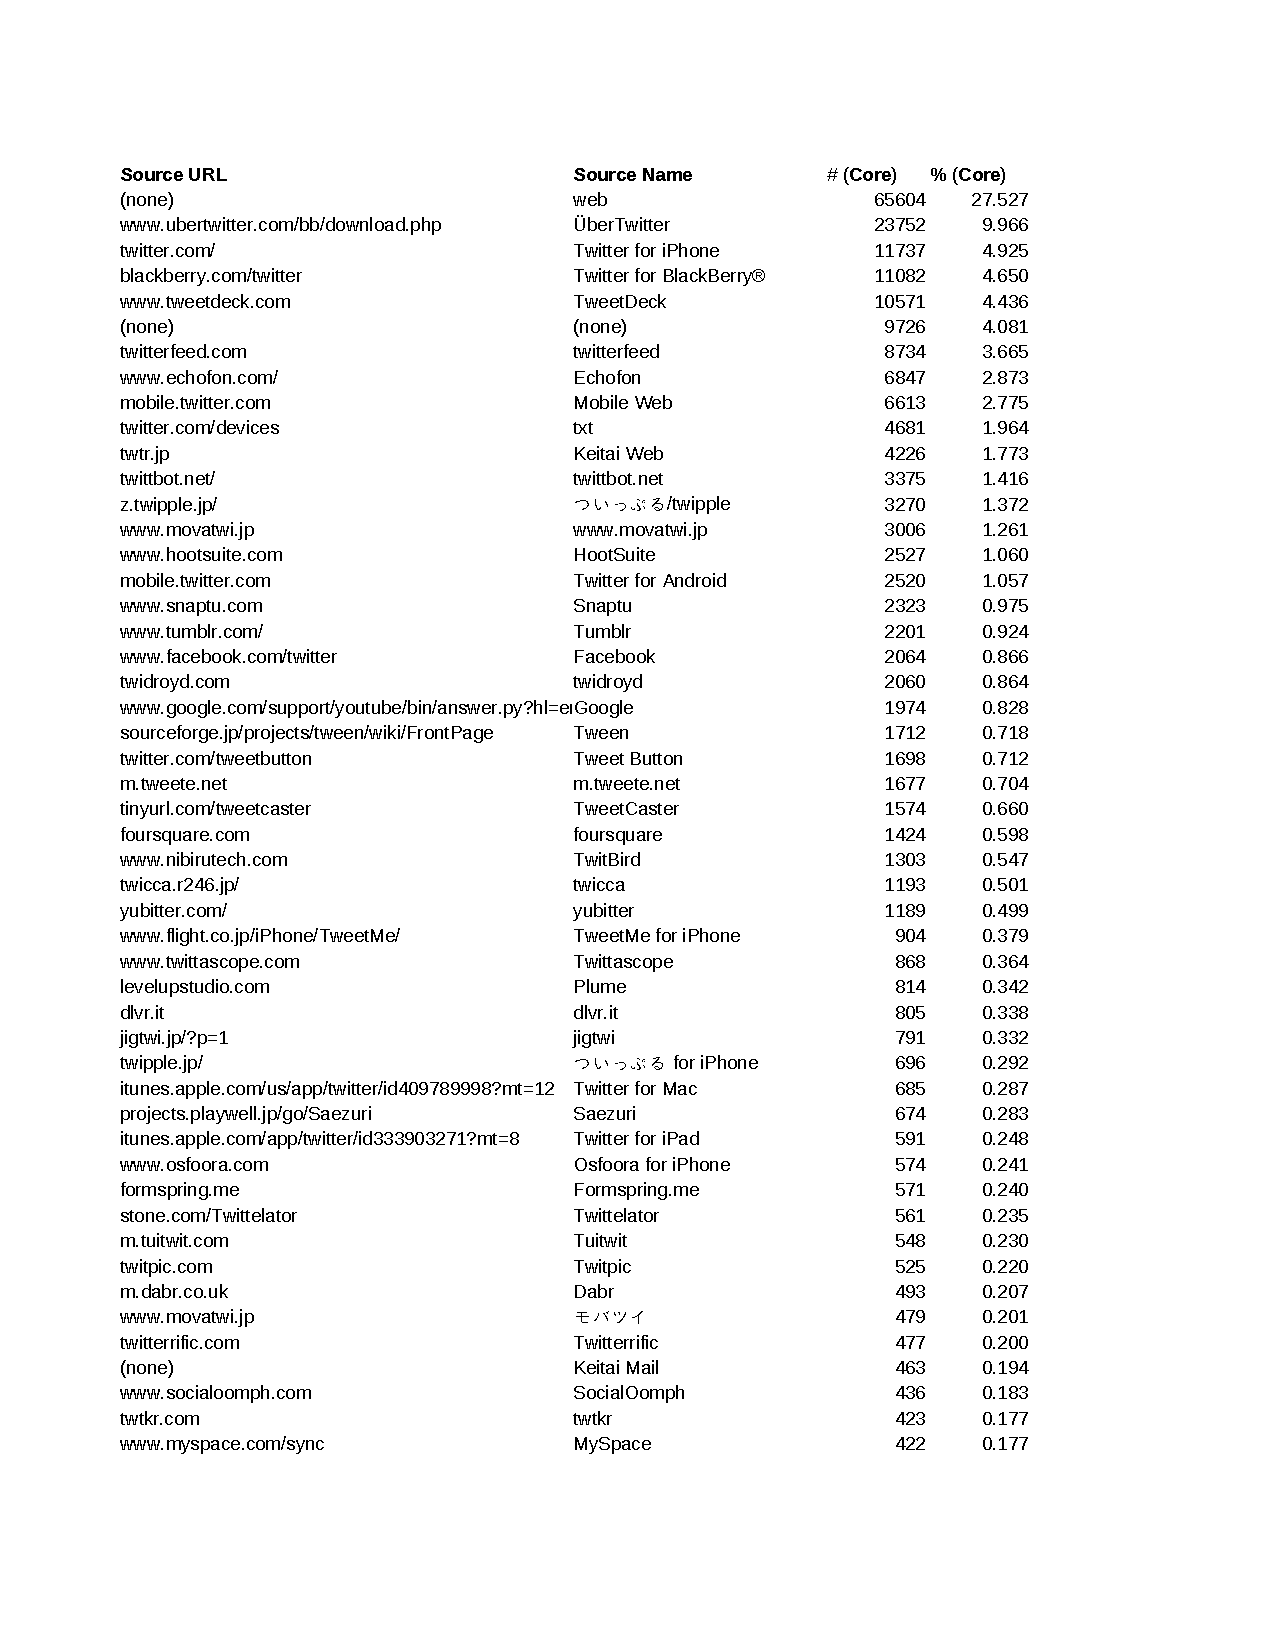
\includegraphics[width=6in,bb=0 0 612 792,keepaspectratio=true]{./sources.pdf}
% sources.pdf: 612x792 pixel, 72dpi, 21.59x27.94 cm, bb=0 0 612 792

\twocolumn
\subsection{Location}
\noindent Location data is entered free-form.  That is, a user can set their location field to anything they want.  In order to use the location data, we need to figure out which locations are not valid, and we need to transform valid locations into a format that can be processed.  For example, we want all users from San Francisco to have a location attribute of \textit{San Francisco, CA, USA}, so that we can easily determine which users share a location.  We are using the Google Maps Geocoding API to make this conversion.  When the API returns more than one result, we can either remove those location from our analysis, try a different method of processing, or try to determine the commonality between multiple results (if, for example, all results are in France, we can use France in our analysis).  When the API returns zero results, we cannot use the location data.\\\\
The Geocoding API has some amount of error.  The returned results are not always a correct transformation of the original location.  We cannot manually examine each result for error, but we do plan to look at a subset of the results and derive a general error rate from that sample.\\\\
The Geocoding API is rate-limited to 2,500 queries per day per IP address.  Google Maps API Premier members can query up to 100,000 per day, but that service starts at \$10,000, so is probably beyond the budget of this project. Yahoo also has a Geocoding API, to which we can make 5,000 calls per day.  However, we would prefer not to complicate the data collection by using both Google and Yahoo services.\\\\
Rate-limiting of Geocoding queries is an issue we need to address urgently.  We either need to find a way to make more requests to the API without breaking the terms of service, or we need to get the information from the Google or Yahoo front-end.  Alternatively, we could design our own location-conversion script, but we see this as non-ideal.



\end{document}
